\chapter{Registracion}

\section{Caracteristicas visuales}

La deteccion de caracteristicas visuales (feature en ingles) es una tecnica muy utiliza en vision por computador para la deteccion, reconocimiento y seguimiento de objetos. Hay dos tareas que deben realizarse para encontrar caracteristicas visuales : la deteccion de un punto de interes (keypoint en ingles), que identifica un area relevante en la imagen, y el computo de un descriptor, que caracteriza a la region. Por lo general, el algoritmo de deteccion identifica regiones en la que su intensidad varia mucho, por ejemplo bordes o esquinas de un objeto, y se selecciona el centro de la region como punto de interes. El descriptor suele representarse como un vector multidimensional que, por lo general, se calcula en base a metricas (como puede ser la orientacion) a partir de los puntos circundantes al keypoint. Es deseable que las caracteristicas detectadas sean invariantes a rotacion, translacion, cambios de iluminacion y escala.

% EXPLICAR PORQUE SE ELIGUEN SURF Y ORB.

\begin{subsection}
{Speeded Up Robust Feature (SURF)}

The Speeded Up Robust Feature (SURF) provides a robust detector and descrip-
tor, that can be used in computer vision tasks like object recognition or 3D
reconstruction. It is partly inspired by the SIFT descriptor, both are using local
gradient histograms. The main difference concerns the performance, lowering the
computational time through an efficient use of integral images for the image con-
volutions, Hessian matrix-based detector (optimized through approximations of the
second order Gaussian partial derivatives, see figure 2.5), and sums of approximated
2D Haar wavelet responses for the descriptor (see figure 2.7). The standard version
of SURF is several times faster than SIFT and claimed by its authors to be more
robust against different image transformations than SIFT.

SURF es un detector y descriptor de caracteristicas \cite{bay2008speeded} en parte inspirado por el descriptor SIFT CITAR[PAPER]. La principal diferencia es la velocidad, siendo la version estandar de SURF un orden magnitud mas rapido que SIFT, y segun sus autores, mas robusto ante diferente tipo de transformaciones.

\begin{subsection} 
{El detector de caracterısticas de SURF}
EL detector de SURF se base en el determinante de la matrix Hessiana. Dada una funcion continua f(x, y), la matrix Hessiana H esta formada por la derivadas parciales de f :

AGREGAR FORMULA DE H.

Siendo el determinante de esta matrix : AGREGAR FORMULA DE DET(H).
A partir del test de la segunda derivada REFERENCIAR, se tiene que si el determinante es positivo se puede clasificar a ese punto de la funcion como un maximo o minimo local, mientras que si es negativo se obtiene que no es un extremo local.

REFERENCIA
[Si la Hessiana es definida positiva en x, entonces f (x) tiene un m ́
ınimo local en x. Si la Hessiana es
definida negativa, entonces f (x) tiene un m ́
aximo local en x. Si la Hessiana tiene autovalores positivos y
negativos, f (x) es un punto de silla. En otro caso el test no aporta informaci ́
on.]

Al aplicar esta teoria al dominio de las imagenes, se sustituye f(x, y)
por la intensidad de los pixeles de la imagen I(x, y) y se reemplaza el calculo de 
las derivadas parciales por la aplicacion de filtros de convolucion. En particular, para calcular las derivadas parciales se pueden utilizar kernels que discretizan las derivadas segundas de la funcion Gaussiana, con Lxx(x, sigma) denotando la evaluacion de derivada parcial. Sin embargo, los autores de SURF proponen una aproximacion a estos kernels por medio de box filters. Como se observa en la figura, los box filters son filtros de convolucion muy simples, que pueden ser aplicados eficientemente utilizando una representacion intermedia de la imagen, la imagen integral \cite{Crow84}.

Para calcular el determinante de la Hessiana por medio de box filters se utiliza una aproximacion, denominada blob response en (x, y, sigma), que se define como : 
AGREGAR FORMULA.

Para encontrar las caracteristicas visuales se utiliza el concepto de espacio de escalas (scale space). El espacio de escalas de una imagen I es una funcion continua, parametrizada en t, que representa un conjunto (infinito) de imagenes, obtenidas a partir de suavizar I, con resultados mas pronunciados a medida que t crece. Tradicionalmente, un scale space se suele implementar como una piramide imagenes donde iterativamente se aplican filtros de suavizado por convolucion y se reduce el tamaño de la imagen. Este metodo se aplica en SIFT, pero es computacionalmente costoso debido al re-escalado de las imagenes. En SURF, se implementa un enfoque diferente, basado en el hecho que la construccion de un box filter no depende del tamaño del mismo, por lo se construye una piramide de filtros para ser utilizados con la imagen original. De esta forma, permite calcular el blob response en varias escalas en paralelo, sin necesidad de re-escalar la imagen. En la figura \ref{fig:scale-space} se ilustra la diferencia entre el enfoque aplicado en SIFT y el propuesto en SURF para la construccion del espacio de escalas.

\begin{figure}[ht]
\centering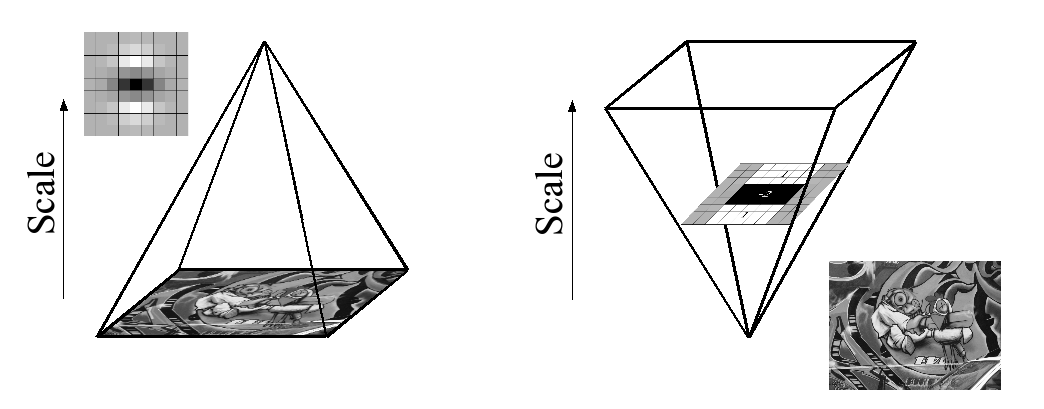
\includegraphics[width=\imsize]
{scale-space}
\caption[Espacio de escalas]
{Enfoques para construir el espacio de escalas. Izquierda : enfoque tradicional donde iterativamente se re-escala la imagen y se suaviza con un filtro Gaussiano de un determinado tamaño. Derecha : enfoque propuesto por SURF donde aplican filtros de diferente tamaño (utilizando la imagen integral) manteniendo la imagen original. Fuente : \cite{bay2008speeded}.}
\label{fig:scale-space}
\end{figure}

El proceso de deteccion SURF se divide en 3 etapas :
\begin{itemize}

\item Filtrado de blob responses : caracteristicas con respuesta por debajo de un umbral se eliminan. Incrementar el umbral reduce la cantidad de caracteristicas detectadas dejando la mas robustas. 

\item Aplicacion del algoritmo de non-maximal suppresion : se compara el pixel candidato con sus 26 vecinos (8 en la escala del candidato y 9 en las escalas superior e inferior) descartandolo cuando su respuesta no es maxima.

\item Interpolacion : se interpolan los datos en la cercania del candidato para obtener una localizacion con precision de subpixel.

\end{itemize}

\end{subsection}

\begin{subsection} 
{El descriptor de SURF}
El descriptor de SURF describe como se distribuye la intensidad de los pixeles vecinos de una caracterisitica encontrada con el detector previamente explicado. El computo del descriptor tiene 2 etapas : la extraccion de la orientacion predominante de la caracteristica y el computo de los componentes del vector utilizando Haar wavelets. \\ Los Haars wavelets son filtros que se utilizan para calcular los gradientes en x y y. Como se observa en la figura \cite{fig:haar-wavelet}, la simplidad de los filtros, permite aplicar la representacion de la imagen integral para implementar la convolucion de forma eficiente.

\begin{figure}[ht]
\centering
\begin{minipage}[h]{.45\textwidth}
\begin{center}
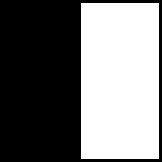
\includegraphics[width=\imsizeS]{haar-wavelet-x}
\end{center}
\end{minipage}
\hfill
\begin{minipage}[h]{.45\textwidth}
\begin{center}
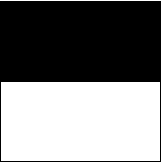
\includegraphics[width=\imsizeS]{haar-wavelet-y}
\end{center}
\end{minipage}
\hfill
\caption[Haar wavelet]{Filtros Haar wavelet utilizados para computar los gradientes en la direccion x (inquierda) e y (derecha). La parte negra representa el valor −1 y la parte blanca +1. Imagen original : \cite{bay2008speeded}.}
\label{fig:haar-wavelet}
\end{figure}

Para extraer la orientacion de una feature se realizan 2 tareas : 

\begin{enumerate}

\item Se computan las respuestas Haar wavelet de tamaño 4 sigma (siendo sigma la escala asociada al punto de interes) en un radio de 6 sigma alrededor de la caracteristica, para obtener las componentes x e y del gradiente. A las respuestas obtenidas se les aplica una Gaussina (con desvicion de 2 sigma) centrada en el punto de interes. Para cada pixel del area circular, se les asocia un punto 2D en el espacio dado por el vector gradiente.

\item Seleccion de la direccion predominante de las respuestas. Se rota una ventana de tamaño pi/3 alrededor del origen de la caracteristica y se suman las componentes de las respuestas dentro de la seccion. El vector resultante con mayor modulo representa la orientacion predominante del punto de interes. El procedimiento se ilustra en la figura \ref{fig:orientacion-surf}.

\end{enumerate}

\begin{figure}[ht]
\centering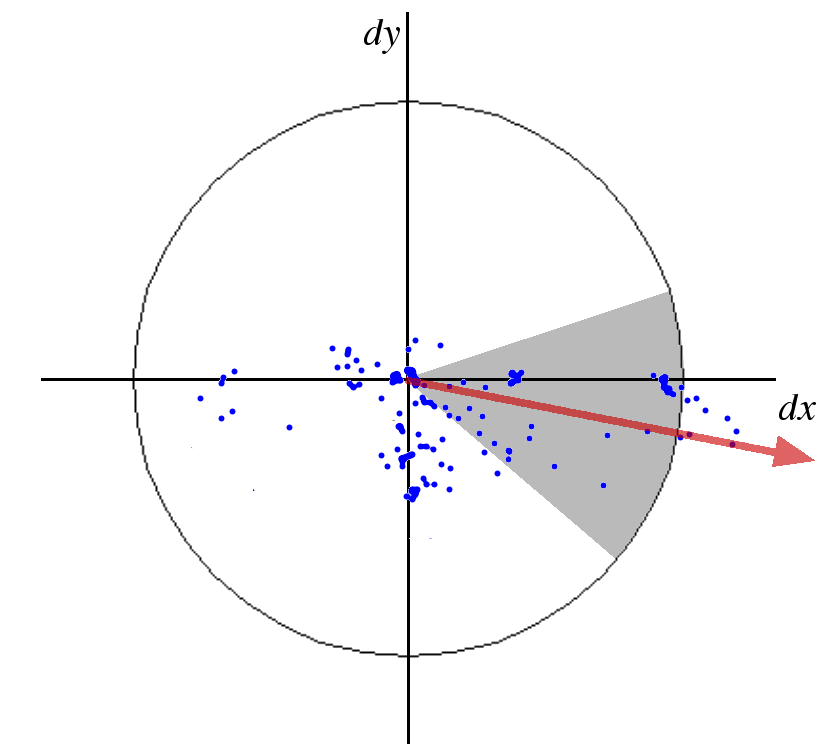
\includegraphics[width=\imsize]
{orientacion-surf}
\caption[Calculo de la orientacion para una caracteristica SURF]
{ La orientacion dominante de la caracteristica se encuentra rotando una ventana de pi/3 alrededor del keypoint, sumando las componentes de las repuestas producidas por los filtros Haar wavelets dentro de la ventana y seleccionando la orientacion del vector resultante con mayor modulo. Fuente : \cite{bay2008speeded}.}
\label{fig:orientacion-surf}
\end{figure}

En algunas aplicaciones, la invarianza de rotacion no es necesaria, lo que permite omitir este paso, dando lugar al denominado Upright SURF (U-SURF).

Para la extraccion de los componentes del descriptor SURF, el primer paso consiste en construir una region rectangular de tamaño 20 sigma alrededor de la caracteristica y orientada en la direccion predominante obtenida en la etapa anterior. La region se divide en 4x4 subregiones rectangulares, y para cada una se computa la respuesta de Haar wavelet de tamaño 2 sigma sobre 25 puntos distribuidos regularmente. Denotando dx y dy, a las respuestas en la direccion x e y respectivamente, se obtiene para cada subregion un vector de la forma v (formula). 
El descriptor resultante se compone por los vectores de cada subregion, por lo que su tamaño es 4 x 4 x 4 = 64 elementos.

\begin{figure}[ht]
\centering
\begin{minipage}[h]{.45\textwidth}
\begin{center}
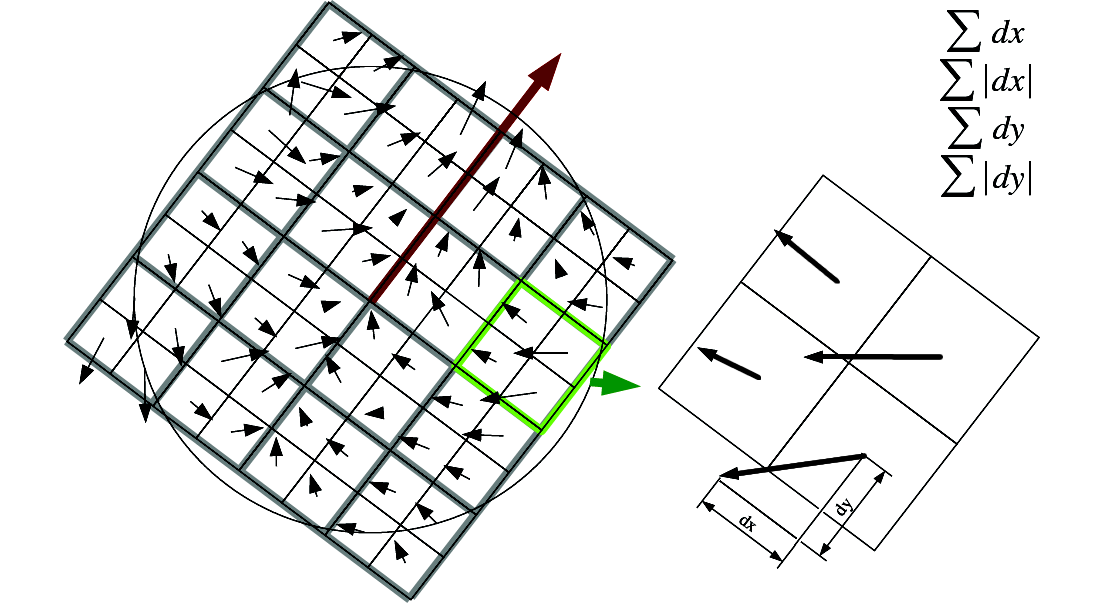
\includegraphics[width=\imsizeS]{grilla-surf}
\end{center}
\end{minipage}
\hfill
\begin{minipage}[h]{.45\textwidth}
\begin{center}
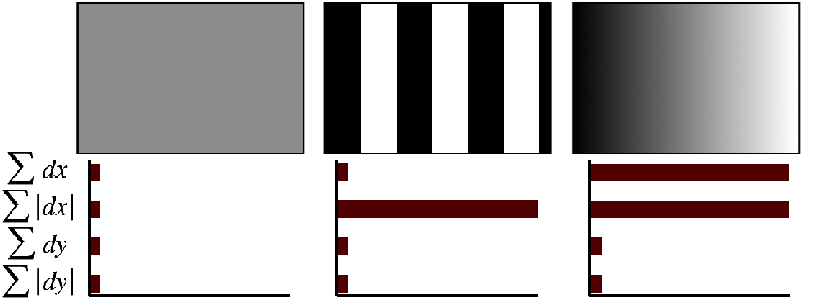
\includegraphics[width=\imsizeS]{histogramas-surf}
\end{center}
\end{minipage}
\hfill
\caption[Calculo del descriptor SURF]
{. Imagen original : \cite{bay2008speeded}.}
\label{fig:haar-wavelet}
\end{figure}


\end{subsection}

\end{subsection}